\documentclass[11pt,a4paper]{article}

\usepackage{fontspec}
\usepackage{amsmath,amssymb,amsfonts}
\usepackage[a4paper,top=2.15cm,bottom=2.2cm,left=2.4cm,right=2.4cm]{geometry}
\usepackage{graphicx}
\usepackage{booktabs}
\usepackage{array,tabularx,longtable,makecell}
\usepackage{float}
\usepackage{caption}
\usepackage{subcaption}
\usepackage{microtype}
\usepackage{setspace}
\usepackage{enumitem}
\usepackage{parskip}
\usepackage{ragged2e}
\usepackage{titlesec}
\usepackage[table]{xcolor}
\usepackage{fancyhdr}
\usepackage{hyperref}
\usepackage{polyglossia}

\setdefaultlanguage{hebrew}
\setotherlanguage{english}

% Academic body typeface with robust fallbacks. Hebrew body text is serif for
% long-form readability; headings remain sans-serif for a clean hierarchy.
\IfFontExistsTF{Libertinus Serif}{
  \setmainfont{Libertinus Serif}
  \newfontfamily\englishfont{Libertinus Serif}[Renderer=HarfBuzz]
}{
  \setmainfont{DejaVu Serif}
  \newfontfamily\englishfont{DejaVu Serif}[Renderer=HarfBuzz]
}
\IfFontExistsTF{Noto Serif Hebrew}{
  \newfontfamily\hebrewfont{Noto Serif Hebrew}[Script=Hebrew,Renderer=HarfBuzz]
}{
  \newfontfamily\hebrewfont{DejaVu Sans}[Script=Hebrew,Renderer=HarfBuzz]
}
\IfFontExistsTF{Noto Sans Hebrew}{
  \newfontfamily\hebrewfontsf{Noto Sans Hebrew}[Script=Hebrew,Renderer=HarfBuzz]
}{
  \newfontfamily\hebrewfontsf{DejaVu Sans}[Script=Hebrew,Renderer=HarfBuzz]
}
\setsansfont{DejaVu Sans}
\setmonofont{DejaVu Sans Mono}
\newfontfamily\hebrewfonttt{DejaVu Sans Mono}[Renderer=HarfBuzz]

\definecolor{academicblue}{RGB}{31,73,112}
\definecolor{deepnavy}{RGB}{25,48,72}
\definecolor{mutedgray}{RGB}{92,101,110}
\definecolor{linegray}{RGB}{218,223,228}
\definecolor{softgray}{RGB}{247,248,250}
\definecolor{tablegray}{RGB}{244,246,248}

\hypersetup{
  colorlinks=true,
  linkcolor=academicblue,
  citecolor=academicblue,
  urlcolor=academicblue,
  pdfencoding=auto,
  psdextra,
  pdftitle={Gaussian HMM לזיהוי משטרי שוק ולחיזוי כיוון יומי},
  pdfauthor={Matan Eshel}
}

\setstretch{1.10}
\setlength{\parindent}{0pt}
\setlength{\parskip}{0.48em}
\setlength{\emergencystretch}{3em}
\raggedbottom
\clubpenalty=10000
\widowpenalty=10000
\displaywidowpenalty=10000

\setlist[itemize]{itemsep=0.22em,topsep=0.3em,leftmargin=1.7em}
\setlist[enumerate]{itemsep=0.22em,topsep=0.3em,leftmargin=1.8em}

\titleformat{\section}
  {\hebrewfontsf\Large\bfseries\color{academicblue}}
  {\thesection}{0.7em}{}
\titleformat{\subsection}
  {\hebrewfontsf\large\bfseries\color{deepnavy}}
  {\thesubsection}{0.6em}{}
\titlespacing*{\section}{0pt}{1.45em}{0.55em}
\titlespacing*{\subsection}{0pt}{1.1em}{0.4em}

\captionsetup{
  font=small,
  labelfont={bf,color=deepnavy},
  textfont={color=mutedgray},
  justification=justified,
  singlelinecheck=false,
  skip=5pt
}
\renewcommand{\arraystretch}{1.16}
\setlength{\tabcolsep}{5pt}
\setlength{\textfloatsep}{1.05em plus 0.2em minus 0.2em}
\setlength{\intextsep}{0.95em plus 0.2em minus 0.2em}

\pagestyle{fancy}
\fancyhf{}
\fancyhead[R]{\hebrewfontsf\small\color{mutedgray} Gaussian HMM לזיהוי משטרי שוק}
\fancyhead[L]{\sffamily\small\color{mutedgray} \LR{Advanced Machine Learning}}
\fancyfoot[C]{\sffamily\small\color{mutedgray}\thepage}
\renewcommand{\headrulewidth}{0.35pt}
\renewcommand{\headrule}{\hbox to\headwidth{\color{linegray}\leaders\hrule height \headrulewidth\hfill}}
\setlength{\headheight}{15pt}

\newcommand{\tech}[1]{\LR{#1}}
\newcommand{\asset}[1]{\LR{#1}}
\newcommand{\pct}[1]{\LR{#1\%}}
\newcommand{\datecode}[1]{\mbox{\textenglish{#1}}}
\newcommand{\code}[1]{\mbox{\textenglish{\texttt{\detokenize{#1}}}}}
\newcolumntype{Y}{>{\RaggedLeft\arraybackslash}X}
\newcolumntype{L}{>{\RaggedRight\arraybackslash}X}
\newcolumntype{C}{>{\centering\arraybackslash}X}

\graphicspath{{../experiments_extended/extended_20260811_121957/}{../experiments_supervised/supervised_20260811_133344/}}

\begin{document}

\begin{titlepage}
\thispagestyle{empty}
\begin{center}
\vspace*{0.9cm}
{\hebrewfontsf\Large\color{mutedgray} המכללה האקדמית להנדסה אפקה \par}
\vspace{0.22cm}
{\hebrewfontsf\large\color{mutedgray} תואר שני במערכות תבוניות \par}

\vspace{1.45cm}
{\color{linegray}\rule{0.82\textwidth}{0.8pt}}\par
\vspace{0.8cm}
{\hebrewfontsf\Huge\bfseries\color{academicblue} Gaussian HMM לזיהוי משטרי שוק ולחיזוי כיוון יומי \par}
\vspace{0.65cm}
\begin{minipage}{0.82\textwidth}
\centering
{\hebrewfontsf\Large\color{deepnavy} ניתוח רב־נכסי, יציבות משטרים והשוואה למודלי בסיס ול־\LR{Supervised ML} \par}
\end{minipage}
\vspace{0.8cm}
{\color{linegray}\rule{0.82\textwidth}{0.8pt}}\par

\vspace{1.35cm}
{\hebrewfontsf\large עבודת גמר בקורס \textbf{שיטות מתקדמות בלמידת מכונה} \par}

\vfill
{\hebrewfontsf\Large\bfseries\color{deepnavy} מתן אשל \par}
\vspace{0.25cm}
{\hebrewfontsf\large מספר סטודנט: \LR{203502802} \par}
\vspace{0.75cm}
{\hebrewfontsf\large\color{mutedgray} אוגוסט 2026 \par}
\vspace{0.75cm}
\end{center}
\end{titlepage}

\pagenumbering{roman}
\begin{abstract}
עבודה זו בוחנת את השימוש ב־\tech{Gaussian Hidden Markov Model (HMM)} בשתי רמות: חיזוי כיוון התשואה ביום הבא, וזיהוי משטרי שוק סמויים בעלי משמעות סטטיסטית. הניסוי הסופי כולל תשעה נכסים מייצגים — \asset{SPY}, \asset{QQQ}, \asset{IWM}, \asset{TLT}, \asset{GLD}, \asset{HYG}, \asset{BTC-USD}, \asset{JPM} ו־\asset{NVDA} — בטווח \datecode{2014-01-01--2024-12-31}. לכל יום מחושבים ארבעה Features: תשואה לוגריתמית, תנודתיות מתגלגלת ל־20 ימים, טווח תוך־יומי ושינוי לוגריתמי בנפח. החלוקה כרונולוגית ומוגנת מזליגה: Train, Validation ו־Test, כאשר preprocessing מותאם על Train בלבד.

לכל נכס נבדקו \(K\in\{2,3,4\}\) וחמישה seeds. בחירת \(K\) ו־seed נעשתה לפי Validation log-likelihood בלבד. בנוסף ל־hard state assignment נבדקה תחזית המבוססת על כל וקטור ה־posterior. המודל הושווה ל־Baselines פשוטים ולשלושה מודלי Supervised ML: Logistic Regression, Random Forest ו־HistGradientBoosting.

מבחינת חיזוי, לא נמצא יתרון עקבי ל־HMM: ממוצע ה־DPA בין תשעת הנכסים היה \pct{54.54} ל־Naive train-mean, \pct{54.14} ל־Logistic Regression, \pct{53.27} ל־Random Forest, \pct{53.06} ל־HMM soft-posterior, \pct{52.49} ל־HistGradientBoosting ו־\pct{52.06} ל־HMM hard-state. לעומת זאת, ברמת ייצוג מבנה השוק התקבלו ממצאים חזקים יותר. ב־SPY, מודל \(K=4\) יצר states בעלי תשואה, volatility, drawdown, range ומשך שהייה שונים מאוד; ה־posterior entropy עלה בצורה חדה סביב מעברי state; מבנה המצבים היה יציב מאוד בין seeds; ומדד VIX, שלא שימש באימון, הפריד בין חלק מהמשטרים. בנוסף נמצא כי הקורלציות בין SPY לנכסים אחרים משתנות כתלות במשטר.

המסקנה המרכזית היא כי בפרויקט זה ה־HMM שימושי יותר כ־\textbf{latent market-state estimator} מאשר כמודל point forecasting ליום הבא. אין בעבודה טענה לרווחיות מסחר או ליתרון סטטיסטי כללי.
\end{abstract}

\textbf{מילות מפתח:} \tech{Hidden Markov Model}, משטרי שוק, \tech{posterior uncertainty}, \tech{directional prediction}, \tech{walk-forward}, \tech{Supervised Learning}, \tech{Reinforcement Learning}.

\clearpage
\tableofcontents
\thispagestyle{plain}
\clearpage
\pagenumbering{arabic}

\section{מבוא ושאלות המחקר}

שוק ההון אינו מתנהג תמיד באותו אופן. יש תקופות שבהן התשואות קטנות והתנודתיות נמוכה, תקופות שבהן השוק נע במהירות ובחוסר יציבות, ולעיתים גם תקופות של ירידות חדות ולחץ. לכן סביר לחשוב על סדרת המחירים לא כתהליך סטטיסטי יחיד וקבוע, אלא כתהליך שעובר בין כמה ``מצבים'' שונים לאורך הזמן.

מודלים מסוג \tech{regime switching} מתארים את הרעיון הזה באמצעות משתנה חבוי, שאינו נצפה ישירות אך משפיע על ההתפלגות של הנתונים שנמדדים בפועל \cite{hamilton1989new}. ב־\tech{Hidden Markov Model (HMM)}, המצב החבוי משתנה לאורך הזמן לפי הסתברויות מעבר, וכל מצב מייצר תצפיות בעלות מאפיינים שונים \cite{rabiner1989tutorial,murphy2012machine}. בהקשר פיננסי, המשמעות היא שהמודל יכול לזהות למשל תקופה שקטה לעומת תקופה תנודתית, גם אם לא סיפקנו לו מראש תוויות בשם ``שקט'' או ``לחוץ''.

השאלה המקורית של הפרויקט הייתה חיזויית: האם \tech{Gaussian HMM} יכול לזהות מצבי שוק סמויים, ולנצל אותם כדי לשפר את חיזוי כיוון התשואה ביום הבא. קיימות עבודות שמיישמות HMM לנתוני מניות ולבעיות חיזוי דומות \cite{catello2023hmm}. עם זאת, לאחר הריצות הראשונות התברר שהסתכלות רק על דיוק החיזוי מפספסת חלק מהמידע שהמודל מספק. גם כאשר ה־DPA אינו גבוה, ייתכן שה־HMM עדיין מזהה מבנה משמעותי של תנודתיות, סיכון והתמדה לאורך זמן.

לכן העבודה הסופית בוחנת שלוש שאלות מחקר נפרדות:

\begin{enumerate}
    \item \textbf{יכולת חיזוי.} האם HMM משפר את חיזוי הכיוון ביום הבא ביחס לכללי ייחוס פשוטים ולמודלי \tech{Supervised Learning} שמקבלים בדיוק את אותם מאפיינים?
    \item \textbf{איכות הייצוג של מצבי השוק.} האם המצבים החבויים נבדלים זה מזה באופן ברור בתשואה, תנודתיות, טווח יומי, התנהגות נפח המסחר, \tech{drawdown}, שכיחות ומשך שהייה?
    \item \textbf{מידע נוסף על סביבת השוק.} האם זהות המצב ורמת אי־הוודאות של המודל קשורות למעברי משטר, למדד \asset{VIX} ולשינויים במבנה הקורלציה בין נכסים?
\end{enumerate}

ההבחנה בין חיזוי לבין ייצוג היא מרכזית בדוח. חיזוי שואל מה יקרה ביום הבא; ייצוג שואל באיזו סביבה סטטיסטית השוק נמצא כעת. אלה שתי יכולות שונות. מטרת העבודה אינה למצוא בכל מחיר ``מודל מנצח'', אלא להבין איזה מידע ה־HMM מצליח לחלץ מהנתונים, היכן הוא אינו מספק יתרון, ומה ניתן להסיק מהתוצאות באופן זהיר.

\section{נתונים, תכונות ופרוטוקול הניסוי}

\subsection{פאנל הנכסים}

כדי לבדוק שהמסקנות אינן תלויות במניה אחת בלבד, נבחר פאנל של תשעה נכסים בעלי מאפיינים שונים. המטרה אינה לבצע בחירת מניות, אלא להפעיל אותה מתודולוגיה על סוגי סיכון שונים ולבדוק האם התנהגות המודל נשארת דומה.

הנתונים נמשכו באמצעות \tech{yfinance} \cite{yfinance} עבור חלון בקשה של \datecode{2014-01-01 - 2024-12-31}. הנכסים הם:

\begin{itemize}
    \item \asset{SPY} - קרן סל המייצגת את שוק המניות האמריקאי הרחב. היא משמשת גם כנכס הייחוס בניתוח הרב־נכסי.
    \item \asset{QQQ} - קרן סל עם משקל גבוה לחברות טכנולוגיה וצמיחה גדולות.
    \item \asset{IWM} - קרן סל המייצגת מניות אמריקאיות קטנות יחסית.
    \item \asset{TLT} - אג"ח ממשלתיות אמריקאיות ארוכות טווח.
    \item \asset{GLD} - זהב.
    \item \asset{HYG} - אג"ח חברות בדירוג גבוה־סיכון יחסית, כלומר \tech{high yield}.
    \item \asset{BTC-USD} - ביטקוין, כנכס אלטרנטיבי בעל תנודתיות גבוהה.
    \item \asset{JPM} - מניה גדולה מסקטור הפיננסים.
    \item \asset{NVDA} - מניית צמיחה בעלת רגישות גבוהה יחסית לשוק.
\end{itemize}

חשוב להבחין בין חלון הבקשה לבין הנתונים שנכנסו בפועל למודל. זמינות הנתונים שונה מעט בין הנכסים, ובפרט סדרת \asset{BTC-USD} מתחילה מאוחר יותר. לכן כל חלוקה ל־\tech{Train}, \tech{Validation} ו־\tech{Test} נעשתה מתוך התצפיות הזמינות בפועל עבור אותו נכס.

ההורדה בוצעה עם \tech{auto\_adjust=False}. כאשר העמודה \tech{Adj Close} הייתה זמינה, היא שימשה לחישובי תשואה ויעד; אחרת נעשה שימוש ב־\tech{Close}. לא בוצעה השלמה מלאכותית של ימים חסרים. שורות עם ערכי \tech{OHLCV} חסרים או לא־סופיים הוסרו, ולאחר יצירת התכונות הוסרו גם שורות שאין להן מספיק היסטוריה לחישוב חלון מתגלגל או שאין עבורן יעד של היום הבא. בניתוח בין נכסים השתמשנו רק בתאריכים שבהם קיימת תצפית בשתי הסדרות המושוות.

\subsection{וקטור התכונות}

בכל יום המודל מקבל תיאור קצר של מצב השוק באותו יום. במקום להזין עשרות אינדיקטורים טכניים, נבחרו ארבע תכונות פשוטות שקל לפרש. הן מנסות לתאר ארבעה היבטים שונים: כיוון התנועה, עוצמת התנודתיות, טווח המסחר בתוך היום ופעילות המסחר.

וקטור התצפית בזמן \(t\) הוא:

\begin{equation}
\mathbf{x}_t = \left[r_t,\; \sigma_t^{(20)},\; R_t,\; \Delta\log V_t\right].
\end{equation}

לכל רכיב יש משמעות ישירה:

\begin{itemize}
    \item \textbf{תשואה לוגריתמית, \(r_t\).} מודדת את שינוי המחיר בין יום \(t-1\) ליום \(t\):
    \begin{equation}
    r_t = \log\left(\frac{P_t}{P_{t-1}}\right).
    \end{equation}
    ערך חיובי מצביע על עלייה וערך שלילי על ירידה.

    \item \textbf{תנודתיות מתגלגלת, \(\sigma_t^{(20)}\).} סטיית התקן של התשואות ב־20 הימים האחרונים. תכונה זו מתארת אם התקופה האחרונה הייתה רגועה או תנודתית.

    \item \textbf{טווח יומי, \(R_t\).} מבוסס על המחיר הגבוה והנמוך של אותו יום. הוא נותן מידע על עוצמת התנועה בתוך יום המסחר, גם אם מחיר הסגירה השתנה מעט.

    \item \textbf{שינוי לוגריתמי בנפח, \(\Delta\log V_t\).} מודד האם נפח המסחר עלה או ירד ביחס ליום הקודם.
\end{itemize}

כל הנתונים שמשמשים לחישוב התכונות של יום \(t\) מגיעים מהעבר ומהיום הנוכחי בלבד. אין שימוש במחיר או בנפח של יום \(t+1\) בעת בניית וקטור הקלט של יום \(t\).

\subsection{יעד החיזוי והחלוקה הכרונולוגית}

משימת החיזוי היא בינארית: בכל יום אנו שואלים האם התשואה של יום המסחר הבא תהיה חיובית או שלילית. כלומר, הקלט מגיע מיום \(t\), ואילו התווית מתייחסת ליום \(t+1\).

היעד מוגדר כך:

\begin{equation}
y_t = \mathbb{1}\left[r_{t+1}\ge 0\right].
\end{equation}

אם התשואה ביום הבא אינה שלילית, מתקבל \(y_t=1\); אחרת מתקבל \(y_t=0\).

בגלל שמדובר בסדרת זמן, אסור לערבב את הדוגמאות באקראי. חלוקה אקראית הייתה עלולה לאפשר למודל ללמוד מתקופה מאוחרת ולבדוק את עצמו על תקופה מוקדמת יותר, מצב שאינו אפשרי בעולם אמיתי. לכן החלוקה היא כרונולוגית, בקירוב:

\begin{itemize}
    \item \pct{70} ראשונים - \tech{Train}, לצורך התאמת המודל.
    \item \pct{15} הבאים - \tech{Validation}, לצורך בחירת תצורת ה־HMM.
    \item \pct{15} אחרונים - \tech{Test}, לצורך הערכה סופית בלבד.
\end{itemize}

לא בוצע \tech{shuffle}. בנוסף, כדי למנוע זליגה בדיוק בגבולות החלוקה, השורה האחרונה של כל חלק מוסרת אם היעד שלה כבר שייך לחלק הבא. כך אף תווית עתידית אינה חוצה את הגבול בין קבוצות הנתונים.

יש להבחין בין שלב בחירת המודל לבין ההתאמה הסופית. בזמן השוואת מועמדי HMM, ה־\tech{scaler} מותאם על \tech{Train} בלבד, כל מועמד מאומן על \tech{Train}, והביצועים שלו נמדדים על \tech{Validation}. רק לאחר שנבחרו מספר המצבים \(K\) וה־\tech{seed}, המודל הנבחר וה־\tech{scaler} מותאמים מחדש על כל המידע שהיה זמין לפני ה־\tech{Test}, כלומר \tech{Train+Validation}. ה־\tech{Test} עצמו נשאר סגור עד שלב ההערכה הסופי.

במודלי \tech{Supervised Learning} נקבעו ה־\tech{hyperparameters} מראש ולא בוצעה בחירה לפי \tech{Validation}. לכן שלושת המודלים האלה אומנו על \tech{Train} בלבד ונבדקו על אותו \tech{Test} כרונולוגי. המשמעות היא שההשוואה בינם לבין ה־HMM אינה משתמשת בדיוק באותה כמות היסטוריה לאימון; נקודה זו מצוינת בהמשך כחלק ממגבלות הניסוי.

\subsection{שחזור ומעקב אחר מקור התוצאות}

כל ריצה נשמרת בתיקייה חדשה יחד עם קובץ \tech{manifest}. הקובץ מתעד את התאריך, גרסת הקוד, גרסאות הספריות, רשימת הנכסים, התכונות, האתחולים והגדרות המודל. כך ניתן לקשר כל מספר בדוח לריצה שממנה הוא הגיע.

ריצת ה־HMM המרכזית היא \code{extended_20260811_121957}, וריצת מודלי ה־\tech{Supervised Learning} היא \code{supervised_20260811_133344}. תוצאות ישנות נשמרו לצורכי ביקורת ושחזור, אך אינן משמשות לטענות המספריות בדוח זה.

\section{מתודולוגיה}

\subsection{מודל מרקוב חבוי}

הרעיון של HMM הוא להניח שמאחורי הנתונים הנצפים קיימת סדרה של מצבים שאיננו רואים ישירות. במקרה שלנו איננו אומרים למודל מראש אילו ימים הם ``רגועים'' או ``לחוצים''. במקום זאת, המודל מנסה להסביר את וקטורי התכונות באמצעות מספר קטן של מצבים חבויים, כאשר לכל מצב יש התפלגות שונה של התצפיות ודפוס שונה של מעבר למצבים אחרים.

נסמן את המצב החבוי ביום \(t\) ב־\(S_t\), כאשר

\begin{equation}
S_t\in\{1,\ldots,K\}.
\end{equation}

הנחת מרקוב מסדר ראשון אומרת שלצורך חיזוי המצב הבא מספיק לדעת את המצב הנוכחי. אין צורך לזכור במפורש את כל רצף המצבים שקדמו לו:

\begin{equation}
P(S_t\mid S_1,\ldots,S_{t-1}) = P(S_t\mid S_{t-1}).
\end{equation}

את הסתברויות המעבר מרכזים במטריצה \(A\). כל איבר במטריצה הוא

\begin{equation}
a_{ij}=P(S_t=j\mid S_{t-1}=i).
\end{equation}

לדוגמה, אם \(a_{33}\) גבוה, המשמעות היא שכאשר המודל נמצא במצב 3 יש סיכוי גבוה שהוא יישאר במצב 3 גם ביום הבא. לכן הערכים שעל האלכסון של מטריצת המעבר מתארים את מידת ההתמדה של כל משטר.

ב־\tech{Gaussian HMM}, וקטור התכונות של כל יום מתואר באמצעות התפלגות גאוסית שתלויה במצב החבוי:

\begin{equation}
\mathbf{X}_t\mid S_t=k \sim \mathcal{N}(\boldsymbol{\mu}_k,\Sigma_k).
\end{equation}

כלומר, לכל מצב \(k\) יש וקטור ממוצעים משלו ומטריצת שונות־קווריאנס משלו. מצב שקט יכול למשל לקבל ממוצע תנודתיות נמוך, בעוד מצב לחוץ יכול לקבל תנודתיות וטווח יומי גבוהים יותר.

בפרויקט נעשה שימוש בספריית \tech{hmmlearn} \cite{hmmlearn} עם מטריצת קווריאנס מלאה. פרמטרי המודל נלמדים באמצעות \tech{Baum-Welch}, שהוא יישום של אלגוריתם \tech{Expectation-Maximization (EM)} \cite{baum1970maximization}. באופן אינטואיטיבי, האלגוריתם חוזר שוב ושוב על שני שלבים: תחילה הוא מעריך את ההסתברות שכל יום שייך לכל מצב; לאחר מכן הוא מעדכן את פרמטרי המצבים והמעברים בהתאם להסתברויות האלה. התהליך נמשך עד שהשיפור ב־\tech{log-likelihood} נעשה קטן והמודל מתכנס.

\subsection{בחירת מספר המצבים}

לפני שרצים על המספרים חשוב להבין מה מחפשים. מעט מדי מצבים עלולים לאחד יחד תקופות שונות מאוד, למשל תקופה רגועה ותקופה תנודתית. יותר מדי מצבים עלולים לפצל את הנתונים לקבוצות קטנות ולא יציבות שקשה לפרש. לכן מספר המצבים \(K\) הוא חלק מהמודל שיש לבחור באופן מבוקר.

לכל נכס נבדקו שלוש אפשרויות: \(K=2\), \(K=3\) ו־\(K=4\). לכל אפשרות בוצעו חמישה אתחולים אקראיים עם ה־\tech{seeds} הבאים: \(42,123,456,789,2026\). הסיבה לריבוי אתחולים היא שאלגוריתם EM יכול להתכנס לפתרונות מקומיים שונים בהתאם לנקודת ההתחלה.

קריטריון הבחירה הראשי היה \tech{Validation log-likelihood}. זהו מדד לשאלה עד כמה המודל שנלמד על \tech{Train} מסביר רצף חדש שלא שימש באימון. ערך גבוה יותר, כלומר פחות שלילי, נחשב טוב יותר. ה־\tech{Test} לא שימש כלל בבחירה.

בנוסף נשמרו \tech{AIC} ו־\tech{BIC} \cite{akaike1974new,schwarz1978estimating}. שני המדדים מאזנים בין איכות ההתאמה לבין מורכבות המודל: מודל עם יותר מצבים יכול להתאים טוב יותר לנתונים, אך הוא גם מכיל יותר פרמטרים ולכן מקבל קנס על מורכבות. ערך נמוך יותר של AIC או BIC עדיף. חשוב להדגיש שמדדים אלה בוחנים התאמה הסתברותית של המודל לנתונים; הם אינם מדדי חיזוי של כיוון היום הבא.

לבסוף נבדקו גם שכיחות השימוש בכל מצב, הנקראת \tech{occupancy}, והיציבות בין אתחולים. מצב שמופיע באחוז זעיר מאוד מהימים עלול להיות אמיתי, למשל מצב משברי נדיר, אך הוא גם עלול להעיד על פיצול יתר. לכן בחירת \(K\) אינה מסתמכת על מספר יחיד בלבד.

\subsection{מצב קשיח לעומת וקטור הסתברויות מלא}

לאחר אימון HMM יש שתי דרכים עיקריות לתאר את המצב של יום מסוים.

בגישה הקשיחה, \tech{hard state}, בוחרים רק את המצב בעל ההסתברות הגבוהה ביותר. לדוגמה, אם ההסתברויות לארבעה מצבים הן \(0.70,0.20,0.08,0.02\), היום יקבל את התווית ``מצב 1''. כל שאר המידע נזרק.

בגישה הרכה, \tech{soft posterior}, שומרים את כל וקטור ההסתברויות. בדוגמה הקודמת נשמר הווקטור המלא ולא רק המצב הראשון. היתרון הוא שהמודל יכול לבטא חוסר ודאות. יום שבו ההסתברויות הן \(0.52,0.45,0.02,0.01\) שונה מאוד מיום שבו הן \(0.98,0.01,0.01,0.00\), גם אם בשני המקרים המצב הקשיח זהה.

בהערכת ה־\tech{Test} השתמשנו ב־\textbf{הסקה סיבתית מהעבר בלבד}. עבור יום \(t\), המודל מקבל את התצפיות עד יום \(t\) ואינו רואה תצפיות עתידיות. וקטור ההסתברויות הוא לכן

\begin{equation}
\gamma_t(k)=P(S_t=k\mid X_{1:t}).
\end{equation}

הסימון \(X_{1:t}\) פירושו כל התצפיות מתחילת הרצף ועד היום הנוכחי. הוא אינו כולל את \(X_{t+1}\) או ימים מאוחרים יותר.

בגרסת התחזית הרכה, תחזית התשואה של היום הבא מחושבת כממוצע משוקלל על פני המצבים לפי \(\gamma_t(k)\). כך, יום שנמצא בגבול בין שני משטרים אינו מטופל כאילו המודל בטוח לחלוטין באחד מהם.

כדי למדוד את מידת אי־הוודאות של הווקטור כולו השתמשנו באנטרופיה מנורמלת:

\begin{equation}
H_t=-\frac{\sum_{k=1}^{K}\gamma_t(k)\log\gamma_t(k)}{\log K}.
\end{equation}

כאשר \(H_t\) קרוב לאפס, כמעט כל ההסתברות מרוכזת במצב אחד ולכן המודל בטוח יחסית. כאשר \(H_t\) גבוה, כמה מצבים מקבלים הסתברויות דומות ולכן המודל פחות בטוח בזהות המשטר.

\subsection{התמדה ומשך שהייה במצב}

אחד המאפיינים החשובים של משטר הוא לא רק איך הוא נראה, אלא גם כמה זמן הוא נוטה להימשך. ב־HMM מסדר ראשון ההסתברות לעזוב מצב מסוים קבועה בכל צעד, כל עוד נשארים באותו מצב. הנחה זו מובילה להתפלגות גאומטרית של משך השהייה.

במילים פשוטות, אם ההסתברות להישאר במצב \(i\) בכל יום היא \(a_{ii}\), אז בכל יום קיימת אותה הסתברות \(1-a_{ii}\) לצאת ממנו. מכאן שהמשך הממוצע הצפוי הוא

\begin{equation}
E[D_i]=\frac{1}{1-a_{ii}}.
\end{equation}

לדוגמה, אם \(a_{ii}=0.95\), משך השהייה הממוצע הצפוי הוא כ־20 ימים. בדוח משווים ערך תיאורטי זה למשך הממוצע שנמדד בפועל ברצף המצבים שפוענח.

ההשוואה הזו בודקת רק את הממוצע, לא את כל צורת התפלגות משכי השהייה. אם רוצים מודל שבו לכל מצב יש התפלגות משך גמישה יותר, אפשר בעתיד להשתמש ב־\tech{Hidden Semi-Markov Model} \cite{bulla2006application}.

\section{ניסויים, \tech{Baselines} ומדדי הערכה}

\subsection{\tech{Baselines} פשוטים}

ה־HMM הושווה תחילה לארבעה כללים פשוטים, כדי לוודא שכל יתרון אינו נובע רק ממגמת שוק בסיסית:

\begin{itemize}
    \item \textbf{\tech{Naive - train mean:}} זהו השם שנשמר ב־artifact. בהערכת ה־Test הסופית התחזית הקבועה מבוססת למעשה על ממוצע \(\texttt{next\_log\_return}\) בכל היסטוריית ה־pre-Test הזמינה, כלומר Train+Validation, לאחר סיום model selection.
    \item \textbf{\tech{Naive persistence:}} מנבא שהכיוון הבא יהיה זהה לכיוון האחרון שנצפה.
    \item \textbf{\tech{Moving Average 5:}} כלל סיבתי המבוסס על ממוצע נע קצר של תשואות זמינות עד היום הנוכחי.
    \item \textbf{\tech{Discrete Markov Chain:}} מודל מעבר נצפה בין Up/Down ללא Hidden States; הפרמטרים נאמדים מהיסטוריית ה־pre-Test בלבד.
\end{itemize}

שלושת ה־Baselines הפשוטים שדורשים אומדן היסטורי משתמשים, כמו ה־HMM הסופי, במידע שהיה זמין לפני תחילת ה־Test. אף אחד מהם אינו משתמש ב־Test targets לצורך התאמה.

\subsection{\tech{Supervised ML Baselines}}

כדי לבדוק אם הקושי החיזויי נובע מבחירת HMM דווקא, נוספו שלושה classifiers המקבלים בדיוק את אותו Feature Vector ואותו split כרונולוגי:

\begin{itemize}
    \item \tech{Logistic Regression} עם \(C=1\) ו־scaling על Train בלבד.
    \item \tech{Random Forest Classifier} עם 500 עצים, depth מרבי 6 ו־minimum leaf size של 10.
    \item \tech{HistGradientBoostingClassifier} עם 200 iterations, learning rate 0.05 ו־15 leaves לכל היותר.
\end{itemize}

ה־hyperparameters נקבעו מראש, ללא search על Validation או Test, ושלושת המודלים הותאמו על Train בלבד. לכן הם משמשים \textbf{Baselines משלימים} ולא תחרות head-to-head מושלמת על כמות זהה של pre-Test observations: ה־HMM, לאחר בחירת \(K\) ו־seed על Validation, עובר refit על Train+Validation. מטרת ההשוואה היא לבדוק האם מודלים ליניאריים ולא־ליניאריים פשוטים מחלצים signal חיזויי ברור מאותם Features, ולא להכריז על classifier אופטימלי.

\subsection{מדדים}

המדד המרכזי לחיזוי כיוון הוא \tech{Directional Prediction Accuracy (DPA)}:

\begin{equation}
\mathrm{DPA}=\frac{1}{N}\sum_{t=1}^{N}\mathbb{1}\left[\operatorname{sign}(\hat r_{t+1})=\operatorname{sign}(r_{t+1})\right].
\end{equation}

למודלים שמחזירים תחזית מספרית לתשואה נמדדו גם MAE ו־RMSE על \textbf{next-day log return}. בנוסף נשמר MAPE על מחיר הסגירה המשתמע מהתחזית, בעיקר כדי לשמור התאמה למדדים שנקבעו בתכנון הפרויקט \cite{hyndman2006another}. MAPE אינו המדד המרכזי כאן: מחיר מחר בדרך כלל קרוב למחיר היום ולכן MAPE על מחיר יכול להיראות נמוך גם עבור Baseline פשוט, בעוד תשואה יומית יכולה להיות קרובה לאפס ולהפוך MAPE על תשואה לבלתי יציב.

עבור מודלי classification נמדדו גם Balanced Accuracy, ROC-AUC, Log Loss ו־Brier Score. המדדים האחרונים חשובים משום ש־Accuracy רגיל עלול להיראות גבוה כאשר שיעור הימים החיוביים גבוה יחסית. עבור classifiers, ה־DPA שקול ל־accuracy של מחלקת הכיוון; עבור המודלים שמחזירים \(\hat r_{t+1}\), הכיוון נגזר מסימן התחזית.

ל־HMM נשמרו בנוסף log-likelihood, AIC/BIC, convergence, occupancy, Transition Matrix, dwell time, posterior confidence וזמן התאמה. מדדים אלה אינם מדדי forecasting; הם מתארים התאמה פנימית, מורכבות ומבנה של המודל. זמן הריצה נשמר לצורך reproducibility ולא שימש לבחירת מודל.

\subsection{ניסויי \tech{Robustness}}

מעבר ל־held-out split נוספו שלושה סוגי בדיקות:

\begin{enumerate}
    \item \textbf{Seed stability:} התאמת כל \(K\) בחמישה seeds והשוואת חלוקת הימים באמצעות \tech{Adjusted Rand Index (ARI)}.
    \item \textbf{Walk-forward על SPY:} שלושה expanding windows, כאשר בכל fold נבנים Train, Validation ו־Test חדשים באופן כרונולוגי.
    \item \textbf{External / cross-asset validation:} השוואת states של SPY ל־VIX, שלא שימש באימון, ובחינת התנהגות נכסים אחרים כתלות ב־SPY state.
\end{enumerate}

בדיקות אלה אינן נועדו לשפר את Test בדיעבד, אלא לבדוק אם המסקנות התיאוריות נשארות סבירות גם מעבר לריצה יחידה.

\section{תוצאות: מבנה המשטרים}

\subsection{בחירת מודל ויציבות}

בריצה המורחבת נבחר \(K=4\) עבור שמונה מתוך תשעת הנכסים; עבור \asset{TLT} נבחר \(K=3\). הבחירה נעשתה לפי Validation log-likelihood בלבד. העובדה ש־\(K=4\) נבחר ברוב הנכסים אינה כשלעצמה הוכחה שזהו מספר states ``אמיתי''; לכן נבדקה גם יציבות בין seeds.

עבור \asset{SPY}, ה־ARI הממוצע בין חמשת ה־seeds ב־\(K=4\) היה 0.995, עם מינימום של 0.992. גם \asset{QQQ} ו־\asset{NVDA} היו יציבים מאוד, עם ARI של כ־0.960 ו־0.984 בהתאמה. לעומת זאת, \asset{BTC-USD} ו־\asset{GLD} היו פחות יציבים ב־\(K=4\), עם ARI של כ־0.553 ו־0.681. לכן המסקנה אינה שכל נכס ``בנוי מארבעה משטרים'', אלא שהמודל העשיר יציב במיוחד בחלק מהנכסים ופחות באחרים.

\begin{figure}[H]
\centering
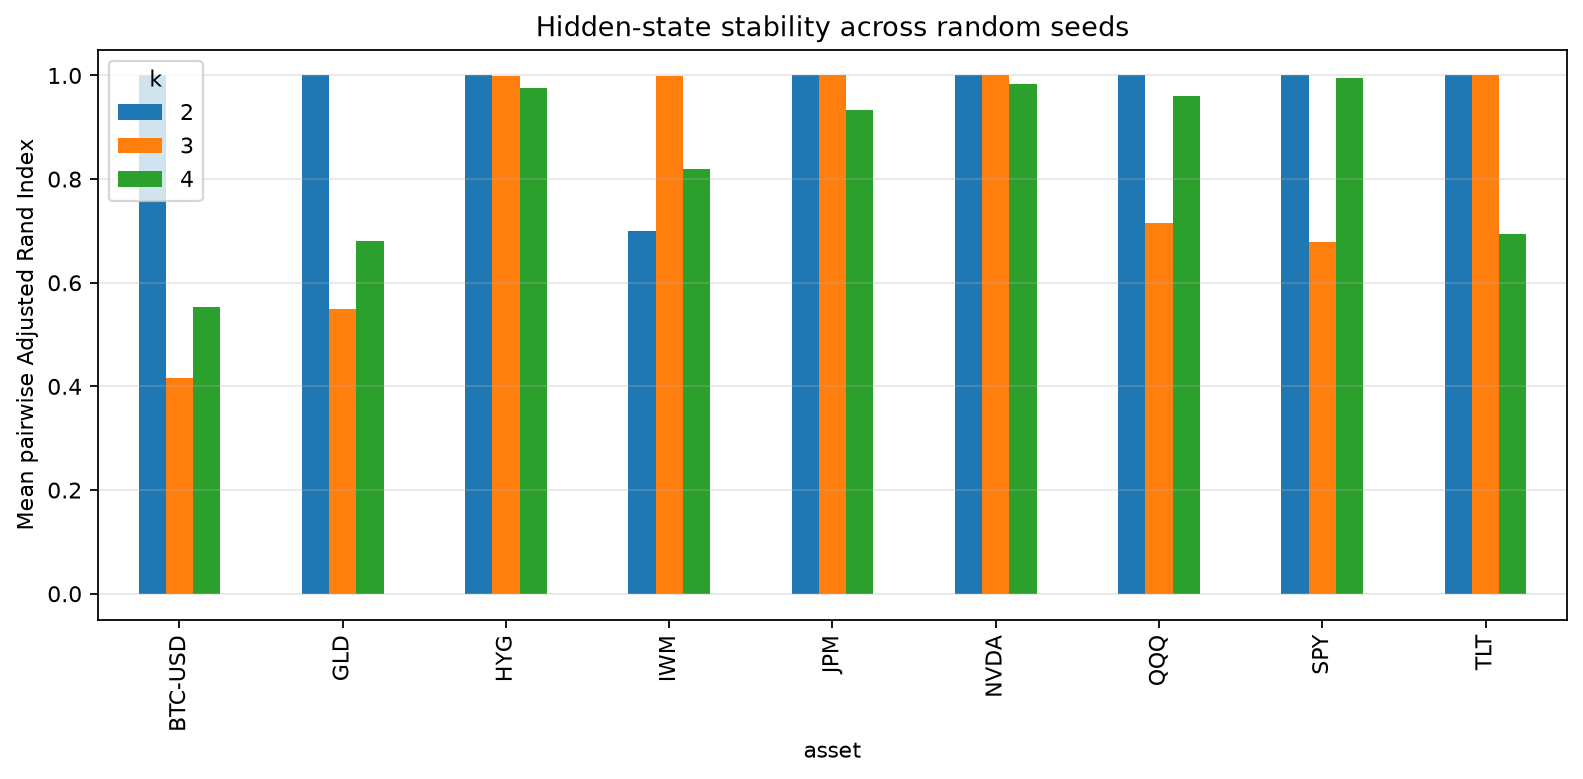
\includegraphics[width=0.88\textwidth]{seed_stability_ari.png}
\caption{יציבות חלוקת ה־states בין seeds לפי ARI. ערכים קרובים ל־1 מצביעים על חלוקה דומה מאוד גם לאחר שינוי initialization.}
\label{fig:seedstability}
\end{figure}

\subsection{פירוש states ב־SPY}

\asset{SPY} משמש מקרה המבחן המרכזי. הטבלה הבאה מסכמת את ארבעת ה־states על פני ההיסטוריה. השמות הם פרשנות post-hoc בלבד; הם לא הוזנו למודל.

\begin{table}[H]
\centering
\small
\begin{tabular}{c l r r r r r r}
\toprule
State & פרשנות & שכיחות & תשואה & Vol. & Range & Mean DD & משך \\
 & & (\%) & יומית (\%) & (\%) & (\%) & (\%) & ימים \\
\midrule
0 & Normal / moderate & 34.31 & 0.053 & 0.692 & 0.841 & -1.72 & 25.0 \\
1 & Calm / low-vol & 25.00 & 0.092 & 0.415 & 0.586 & -0.42 & 32.4 \\
2 & Rare stress / crisis-like & 4.46 & -0.265 & 3.409 & 3.614 & -15.28 & 8.0 \\
3 & Persistent high-vol & 36.23 & 0.039 & 1.239 & 1.497 & -8.11 & 35.2 \\
\bottomrule
\end{tabular}
\caption{מאפייני states של SPY. Vol. היא סטיית תקן יומית ו־Mean DD הוא drawdown ממוצע.}
\label{tab:spystates}
\end{table}

State 2 בולט במיוחד: הוא נדיר, בעל תשואה יומית ממוצעת שלילית, volatility של כ־\pct{3.41}, daily range של כ־\pct{3.61}, mean drawdown של כ־\pct{-15.3} ו־worst drawdown של כ־\pct{-33.7}. לעומתו State 1 הוא state שקט עם volatility של כ־\pct{0.42} ו־drawdown קטן יחסית. זו הפרדה שמצדיקה לדבר על משטרים סטטיסטיים שונים, גם אם אין להם labels כלכליים חד־משמעיים.

\begin{figure}[H]
\centering

\includegraphics[width=0.95\textwidth]{SPY/test_price_by_regime.png}
\caption{מחיר SPY בתקופת ה־Test צבוע לפי ה־state הדומיננטי. הרצפים המתמשכים ממחישים שהמודל אינו מחליף state באופן אקראי בכל יום.}
\label{fig:spyregimes}
\end{figure}

\subsection{Posterior uncertainty סביב מעברים}

ה־posterior confidence הממוצע ב־SPY הוא כ־\pct{96.6}. עם זאת, ה־entropy הממוצע בימי state switch הוא 0.307 לעומת 0.054 בלבד בימים ללא switch. גם בחלון של יום לפני/אחרי מעבר מתקבל entropy ממוצע של כ־0.236. לעומת זאת, המתאם בין entropy לבין absolute return הוא רק 0.027, והמתאם עם rolling volatility הוא כ־-0.076.

מכאן עולה ממצא חשוב: posterior entropy אינו פשוט proxy נוסף ל־volatility. הוא מתאר בעיקר \textbf{אי־ודאות של המודל לגבי גבול בין regimes}. כלומר ה־HMM מספק לא רק state label אלא גם מדד של confidence במצב הנוכחי.

\begin{figure}[H]
\centering

\includegraphics[width=0.95\textwidth]{SPY/posterior_entropy_timeline.png}
\caption{Posterior entropy לאורך תקופת ה־Test של SPY. קפיצות באנטרופיה מופיעות בעיקר סביב שינויי state.}
\label{fig:entropy}
\end{figure}

\subsection{External validation מול VIX}

ה־VIX לא שימש Feature ולא השתתף באימון. לכן הוא משמש בדיקת post-hoc חיצונית. בתקופת החפיפה של 412 ימי Test, State 1 של SPY היה קשור ל־VIX ממוצע של 12.96, State 0 ל־15.34 ו־State 3 ל־18.55. ב־State 3 כ־\pct{26.1} מהימים היו מעל VIX=20, לעומת \pct{6.15} ב־State 0 ואפס ב־State 1.

\begin{figure}[H]
\centering
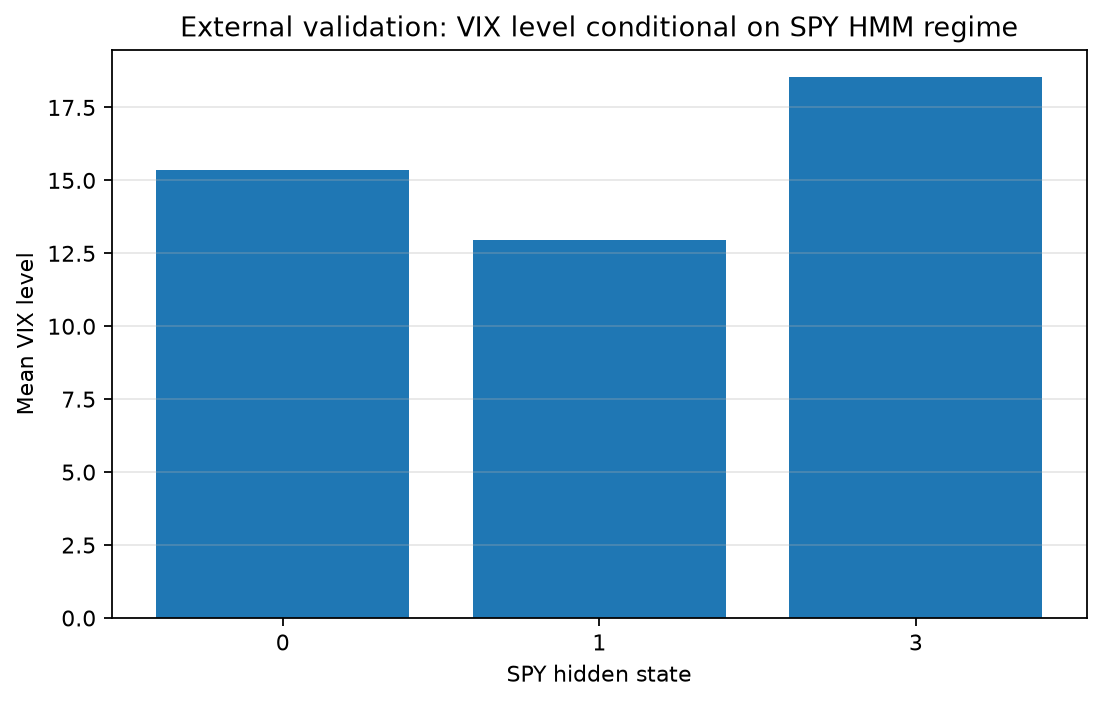
\includegraphics[width=0.78\textwidth]{vix_by_spy_regime.png}
\caption{רמת VIX לפי state של SPY. VIX אינו חלק מווקטור התכונות ולכן משמש אינדיקציה חיצונית לפרשנות המשטרים.}
\label{fig:vix}
\end{figure}

State 2 הנדיר לא הופיע בחפיפה זו ולכן אי אפשר להשתמש ב־VIX כדי לאמת אותו בתקופת ה־Test. בנוסף, entropy עצמו כמעט אינו מתואם עם רמת VIX, ולכן אין לזהות בין ``אי־ודאות של ה־HMM'' לבין ``פחד בשוק''.

\subsection{Cross-asset behavior}

כדי לבדוק האם state של SPY משקף מצב שוק רחב יותר, חושבו סטטיסטיקות של נכסים אחרים מותנות ב־SPY state. ב־State 3 הקורלציה עם SPY מגיעה לכ־0.978 ב־QQQ, 0.773 ב־HYG, 0.631 ב־BTC-USD, 0.680 ב־JPM ו־0.769 ב־NVDA. באותו state, TLT נמצא בקורלציה קרובה לאפס ואף מעט שלילית (-0.044).

\begin{table}[H]
\centering
\small
\begin{tabular}{l r r r}
\toprule
Asset & Corr. State 0 & Corr. State 1 & Corr. State 3 \\
\midrule
\asset{QQQ} & 0.924 & 0.849 & 0.978 \\
\asset{IWM} & 0.733 & 0.240 & 0.879 \\
\asset{TLT} & 0.213 & 0.265 & -0.044 \\
\asset{HYG} & 0.636 & 0.515 & 0.773 \\
\asset{BTC-USD} & 0.207 & 0.329 & 0.631 \\
\asset{JPM} & 0.435 & 0.106 & 0.680 \\
\asset{NVDA} & 0.575 & 0.548 & 0.769 \\
\bottomrule
\end{tabular}
\caption{קורלציה עם SPY כתלות ב־Hidden State של SPY בתקופת ה־Test.}
\label{tab:crossasset}
\end{table}

תוצאה זו מחזקת את הפרשנות של ה־HMM כ־latent market-state estimator: ה־state אינו רק תיאור של תנודתיות SPY, אלא מתקשר גם לשינוי במבנה התלות בין asset classes.

\section{תוצאות: חיזוי יום־קדימה}

\subsection{תמונה כללית}

טבלה \ref{tab:meanDPA} מציגה את ממוצע ה־DPA הבלתי־משוקלל בין תשעת הנכסים. התוצאה החשובה ביותר היא שאין מודל אחד שמציג יתרון חיזויי עקבי.

\begin{table}[H]
\centering
\begin{tabular}{l r}
\toprule
Model & Mean DPA (\%) \\
\midrule
Naive - train mean & 54.54 \\
Logistic Regression & 54.14 \\
Random Forest Classifier & 53.27 \\
Gaussian HMM - soft posterior & 53.06 \\
HistGradientBoostingClassifier & 52.49 \\
Gaussian HMM - hard state & 52.06 \\
\bottomrule
\end{tabular}
\caption{ממוצע DPA בין תשעת הנכסים. הממוצע אינו שקול למבחן מובהקות ואינו מוכיח עליונות כללית של אף מודל.}
\label{tab:meanDPA}
\end{table}

\begin{figure}[H]
\centering
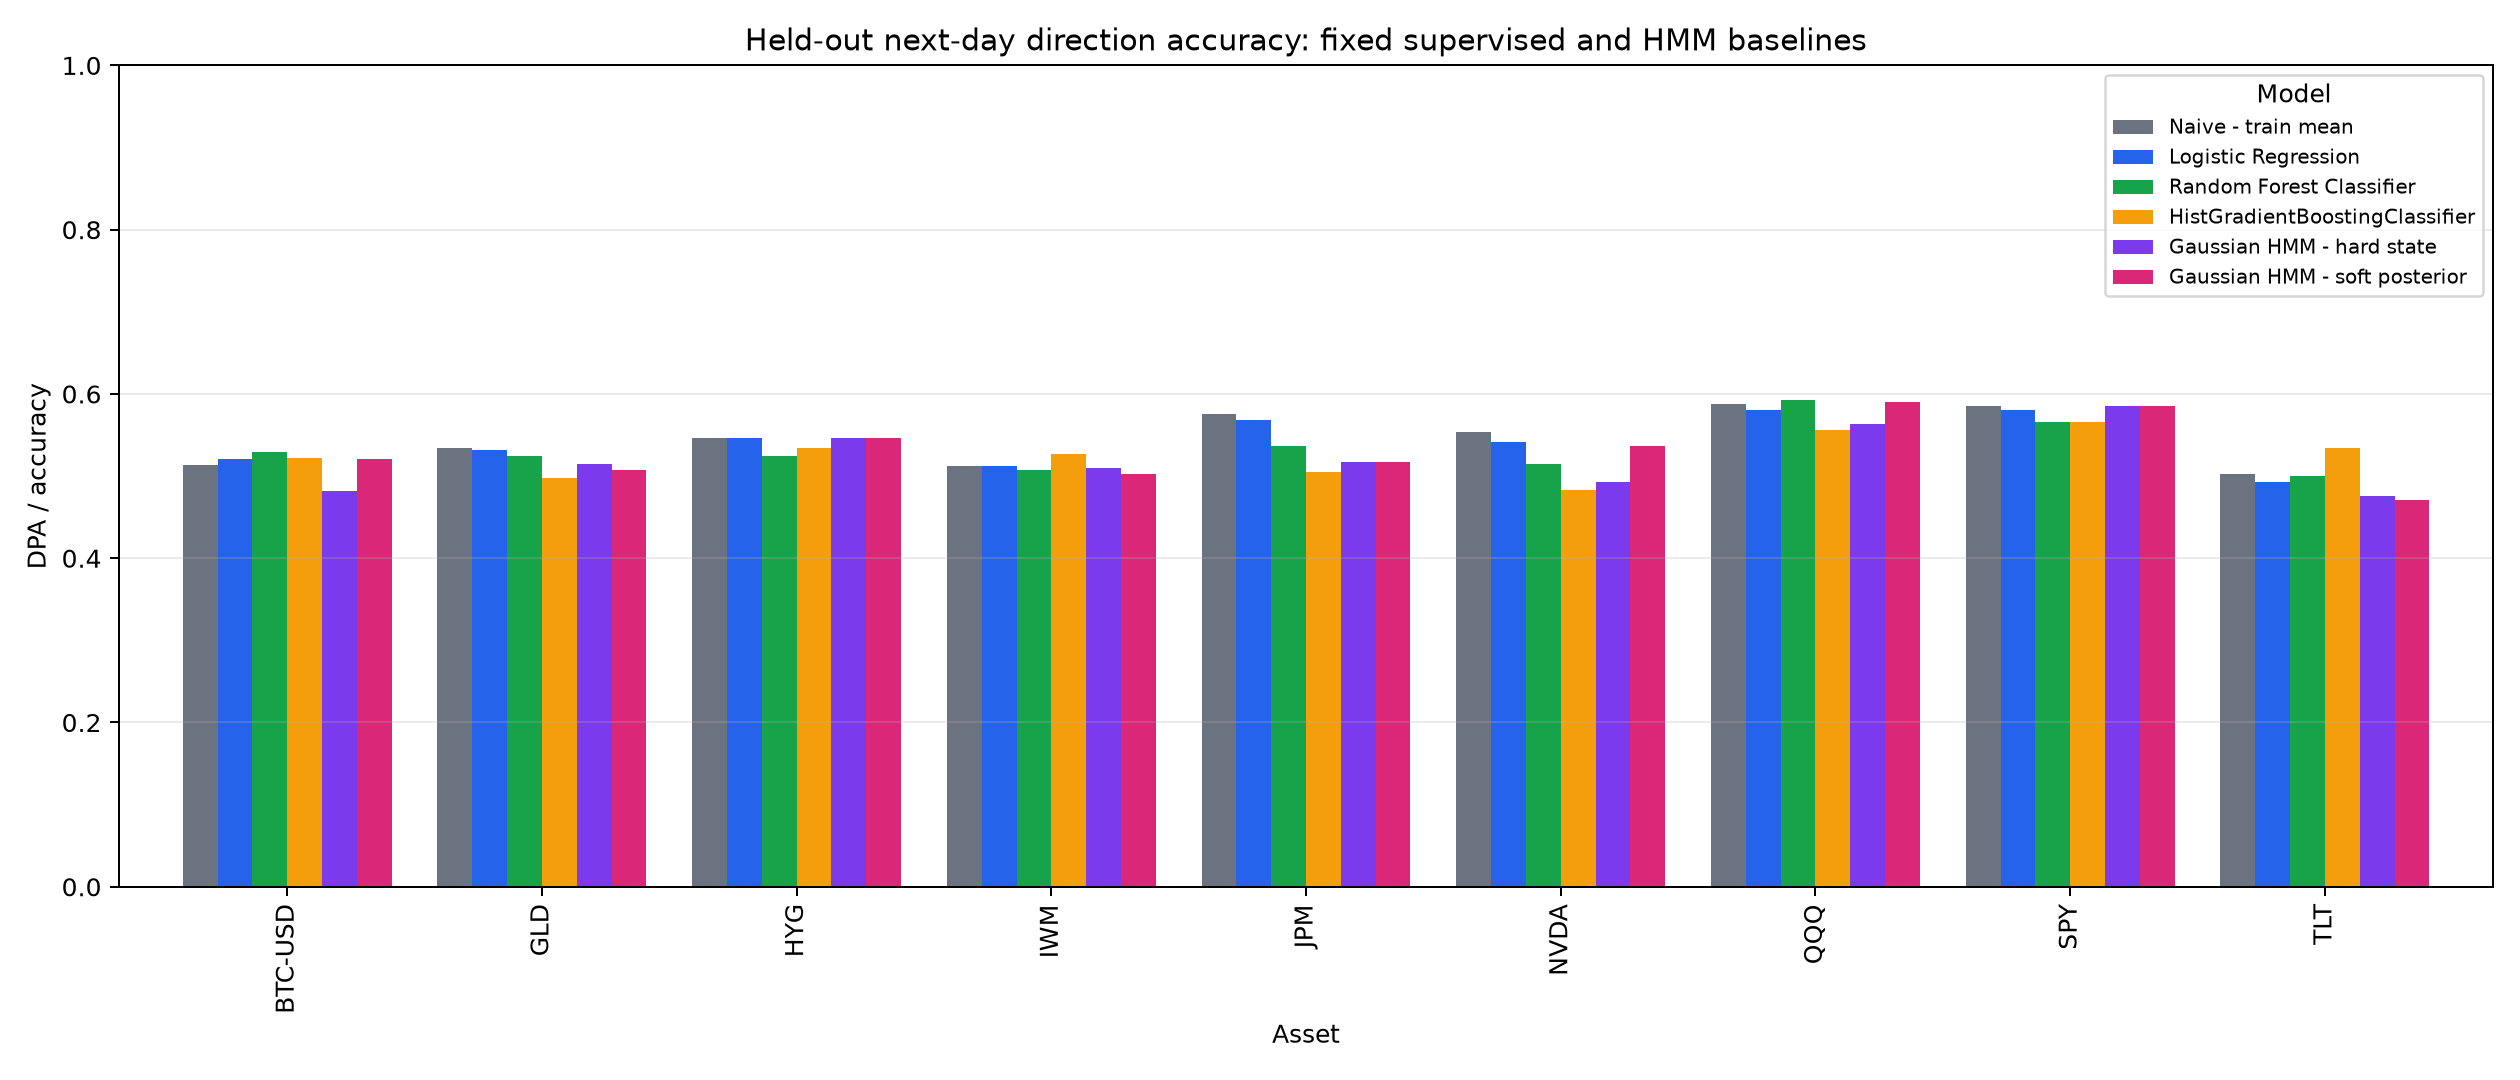
\includegraphics[width=0.98\textwidth]{dpa_comparison_all_assets.png}
\caption{השוואת DPA בין Baseline, שלושת מודלי ה־Supervised ML ו־HMM hard/soft לכל נכס.}
\label{fig:dpaall}
\end{figure}

\subsection{תוצאות לפי נכס}

יש כמה מקרים מקומיים מעניינים. ב־\asset{QQQ}, Random Forest השיג \pct{59.22}, soft HMM השיג \pct{58.98}, וה־Naive baseline \pct{58.74}. ב־\asset{BTC-USD}, Random Forest השיג \pct{52.94} וה־soft HMM \pct{52.05}, לעומת \pct{51.34} ל־Naive. לעומת זאת, ב־\asset{JPM} ה־Naive הגיע ל־\pct{57.52} בעוד soft HMM הגיע ל־\pct{51.70}. ב־\asset{TLT}, HistGradientBoosting היה הטוב ביותר מבין המודלים שנבדקו עם \pct{53.40}, בעוד soft HMM הגיע ל־\pct{47.09}.

הפיזור הזה חשוב יותר מהדירוג הממוצע: HMM אינו נכשל בכל נכס, אך גם אינו מנצח בצורה יציבה. אותו דבר נכון למודלי ה־Supervised ML. לכן אין evidence לכך שה־Feature Vector הנוכחי מכיל signal חזק ועקבי לחיזוי next-day direction.

\subsection{למה DPA לבדו עלול להטעות}

ב־\asset{SPY}, למשל, Naive train-mean ו־HMM מגיעים ל־DPA של כ־\pct{58.50}. עם זאת, Logistic Regression מגיע ל־DPA של \pct{58.01} אך Balanced Accuracy של כ־\pct{49.6} ו־ROC-AUC של כ־\pct{47.3}. Random Forest משיג ROC-AUC של כ־\pct{50.4}. כלומר חלק ניכר מה־Accuracy נובע מחוסר איזון בין ימי Up ו־Down, ולא מיכולת חזקה לדרג ימים לפי הסתברות לעלייה.

זו הסיבה שבדוח לא מתייחסים ל־DPA מעל \pct{50} כהוכחה אוטומטית ל־predictive edge. מודל שמנבא את המחלקה הנפוצה יכול לקבל Accuracy סביר גם בלי להבין את דינמיקת היום הבא.

\subsection{Hard state לעומת Soft posterior}

בממוצע, soft HMM משיג \pct{53.06} לעומת \pct{52.06} ל־hard-state. הפער קטן, אך הוא עקבי עם האינטואיציה שלפיה שימוש בכל וקטור ה־posterior שומר מידע שנזרק ב־argmax. לדוגמה, ב־\asset{QQQ} hard HMM הגיע ל־\pct{56.31} בעוד soft HMM הגיע ל־\pct{58.98}; ב־\asset{BTC-USD} הפער גדול יותר, \pct{48.13} לעומת \pct{52.05}. מנגד קיימים גם נכסים שבהם soft אינו משפר.

לכן המסקנה אינה ש־soft posterior ``פותר'' את forecasting, אלא שהוא דרך הגיונית יותר לנצל posterior uncertainty מאשר hard assignment כאשר משתמשים ב־HMM לתחזית.

\subsection{Walk-forward robustness על SPY}

שלושת ה־walk-forward folds מציגים תמונה מעורבת. soft HMM השיג בהתאמה \pct{50.36}, \pct{51.82} ו־\pct{60.22}; Naive train-mean השיג \pct{48.54}, \pct{52.92} ו־\pct{59.85}. הממוצע הוא \pct{54.14} ל־soft HMM לעומת \pct{53.77} ל־Naive, אך HMM אינו מנצח בכל fold והפער הכולל קטן.

\begin{figure}[H]
\centering
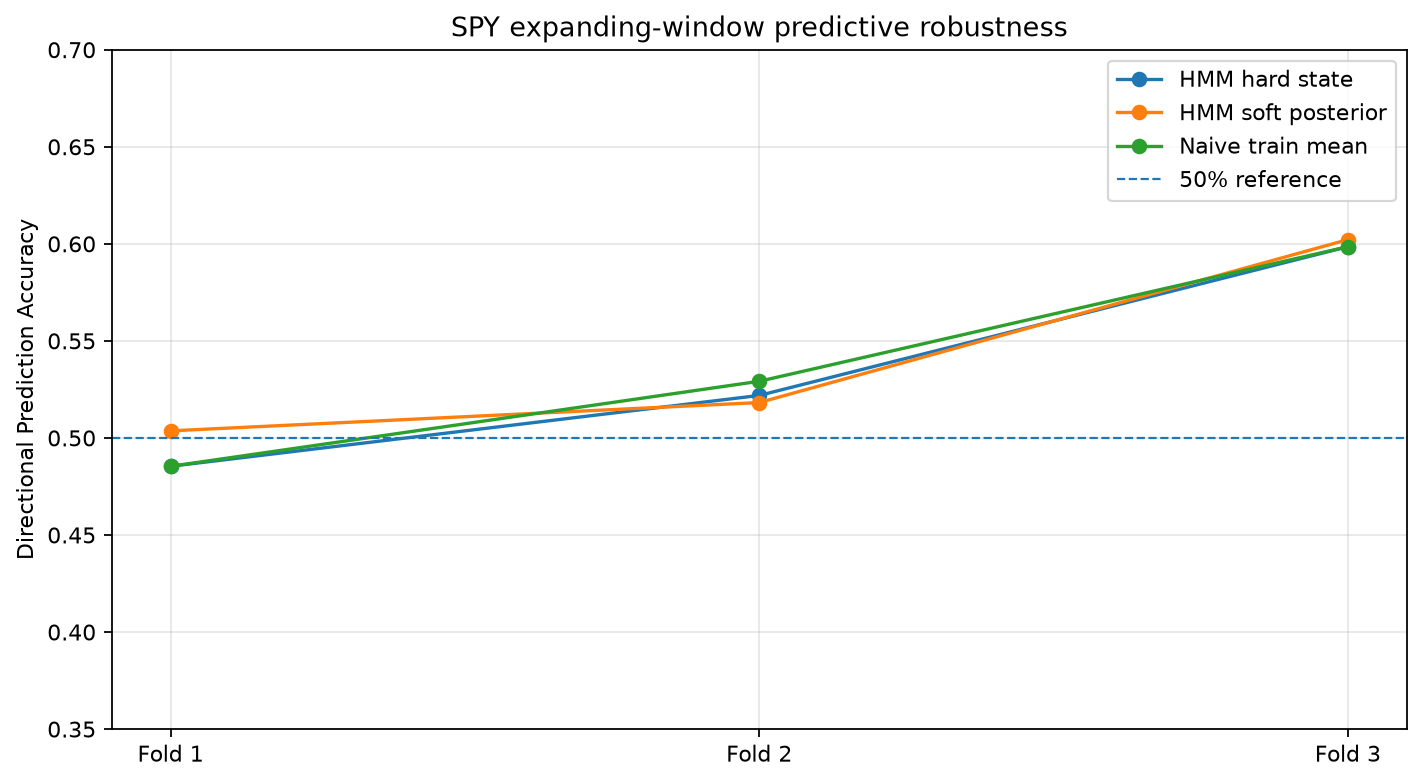
\includegraphics[width=0.82\textwidth]{walk_forward_dpa.png}
\caption{DPA בשלושה expanding walk-forward folds על SPY. ה־HMM אינו מפגין יתרון עקבי בין התקופות.}
\label{fig:walkforward}
\end{figure}

בדיקת ה־walk-forward מחזקת את הצורך בניסוח זהיר: ייתכן שמידע על regime מסייע בתקופות מסוימות, אך לא נמצא predictive advantage יציב שניתן להכליל לכל תקופה.

\section{דיון}

התוצאה המרכזית של העבודה אינה שה־HMM ``מנבא את השוק''. להפך: גם HMM, גם מודלי \tech{Supervised Learning} וגם כללי ייחוס פשוטים מתקשים להפיק אות עקבי לחיזוי היום הבא מתוך ארבעת המאפיינים שנבדקו. דווקא התוצאה הזו מחדדת את ההבדל בין שתי שאלות שונות: האם המודל מנבא היטב, והאם הוא מייצג היטב את מצב השוק.

\subsection{מדוע חיזוי יום קדימה נשאר קשה?}

חיזוי סימן התשואה של יום בודד הוא בעיה רועשת מאוד. התנודתיות של השוק, הטווח היומי והפעילות במסחר יכולים לתאר היטב את רמת הסיכון, אבל אינם בהכרח קובעים אם המחיר יעלה או ירד מחר. לכן ייתכן שמאפיין יהיה שימושי מאוד לזיהוי ``סביבה תנודתית'' בלי להיות שימושי לחיזוי הכיוון ביום הבא.

העובדה שגם \tech{Logistic Regression}, \tech{Random Forest} ו־\tech{HistGradientBoosting} אינם מציגים יתרון עקבי תומכת בפרשנות שהקושי אינו ייחודי ל־HMM. במילים אחרות, לא נראה שמודל סיווג אחר מצליח לחלץ מהתכונות הקיימות אות ברור שה־HMM מפספס.

בנוסף, DPA מושפע מאיזון המחלקות. אם בתקופה מסוימת יש יותר ימי עלייה, כלל פשוט שמנבא עלייה לעיתים קרובות יכול להשיג תוצאה מעל \pct{50}. לכן נעשה שימוש גם ב־\tech{Balanced Accuracy} וב־\tech{ROC-AUC}. ברוב הנכסים מדדים אלה נשארו קרובים ל־\pct{50}, ולכן אין בסיס לטעון שקיים אות חיזויי חזק.

\subsection{מה ה־HMM כן מוסיף?}

כאן נמצא הערך המרכזי של המודל. גם אם איננו יודעים לחזות בביטחון אם מחר יהיה יום חיובי או שלילי, עדיין שימושי לדעת אם אנחנו נמצאים כרגע בתקופה שקטה, בתקופה תנודתית או בסביבה דמוית לחץ. מידע כזה מתאר את \textbf{ההקשר} שבו התשואה הבאה תתרחש.

HMM עושה בדיוק זאת: הוא בונה ייצוג מפורש של מצב חבוי ושל דינמיקת המעבר בין מצבים. עבור \asset{SPY}, ארבעת המצבים נבדלים בו־זמנית בתשואה, תנודתיות, טווח יומי, \tech{drawdown} ומשך שהייה. לכן המודל אינו רק מחלק ימים לפי ``תנודתיות גבוהה או נמוכה'', אלא יוצר תיאור רב־ממדי של סביבת השוק.

נוסף לכך, וקטור ה־\tech{posterior} מספק מידע על מידת הביטחון של המודל. רוב הזמן ההסתברות מרוכזת במצב אחד, אך סביב גבולות בין מצבים היא מתפזרת יותר. כפי שהוסבר קודם, הקשר בין אנטרופיה לבין מעבר מצב הוא בחלקו מכני משום ששני המדדים נגזרים מאותו \tech{posterior}. לכן אין לראות בו אימות חיצוני. עם זאת, הוא כן מספק מדד פנימי שימושי לשאלה עד כמה ההחלטה על זהות המשטר חד־משמעית.

הראיות החיצוניות מגיעות משני מקורות אחרים. ראשית, \asset{VIX}, שלא שימש באימון, מקבל רמות שונות במצבים שונים. שנית, הקורלציות בין \asset{SPY} לנכסי סיכון אחרים משתנות לפי המצב. שתי התוצאות הן תיאוריות בלבד, אך הן מראות שהמצב החבוי קשור למאפיינים רחבים יותר של השוק ולא רק לאחד המשתנים שהוזנו ישירות למודל.

מכאן מגיע הביטוי \tech{conditional market context}. בעברית, הכוונה היא שה־HMM מספק הקשר מותנה למצב השוק: במקום לשאול רק ``האם מחר תהיה עלייה?'', אפשר לשאול ``באיזה סוג סביבה אנחנו נמצאים עכשיו, כמה המודל בטוח בכך, ועד כמה ההתנהגות של נכסים אחרים משתנה בסביבה הזאת?''. זו יכולת שאינה נמדדת ישירות באמצעות DPA.

\subsection{עושר המודל מול יציבות}

מספר גדול יותר של מצבים מאפשר למודל לתאר מבנה עשיר יותר, אך הוא גם מגדיל את הסיכון למצבים נדירים או לפתרונות שתלויים באתחול. זהו מתח טבעי בין גמישות לבין יציבות.

בממצאים שלנו, \(K=2\) נוטה להיות יציב מאוד אך גס יחסית. \(K=4\) מאפשר הפרדה מפורטת יותר, וב־\asset{SPY}, \asset{QQQ} ו־\asset{NVDA} הוא גם יציב מאוד בין אתחולים. לעומת זאת, ב־\asset{BTC-USD} וב־\asset{GLD} היציבות נמוכה יותר. לכן אין הצדקה לקבוע מראש שמספר מצבים אחד מתאים לכל נכס או לכל תקופה.

\subsection{מדוע לא קראנו למצבים שוק שורי ושוק דובי (\tech{Bull/Bear})?}

בשפה פיננסית, \tech{bull market} הוא בדרך כלל שוק בעל מגמת עלייה מתמשכת, ואילו \tech{bear market} מתאר תקופה ממושכת של ירידות. אלה מושגים כלכליים מוכרים, אך ה־HMM שלנו לא אומן לזהות אותם באופן ישיר.

המצבים בפרויקט נלמדים מתוך ארבע תכונות יומיות, וההבדלים הבולטים ביניהם קשורים בעיקר לתנודתיות, לטווח היומי, ל־\tech{drawdown} ולהתמדה. מצב יכול להיות תנודתי מאוד ועדיין לקבל תשואה ממוצעת חיובית, ולכן תווית ``Bear'' עלולה להיות מטעה. באותו אופן, מספר מצב כמו 0 או 3 הוא שרירותי לחלוטין ויכול להתחלף בין ריצות.

לכן נעשה שימוש בשמות תיאוריים זהירים כמו \tech{Calm / low-vol} או \tech{Rare stress / crisis-like} רק לאחר בחינת הסטטיסטיקות. לדוגמה, מצב 2 של \asset{SPY} מכונה דמוי־משבר משום שהוא נדיר, בעל תשואה ממוצעת שלילית, תנודתיות גבוהה ו־\tech{drawdown} עמוק. גם שם זה הוא פרשנות ולא אמת חיצונית שניתנה למודל.

\subsection{משך המשטר ומה משמעות ה־HMM במקרה שלנו?}

ההשוואה בין משך השהייה התיאורטי, \(1/(1-a_{ii})\), לבין משך השהייה שנמדד בפועל לא חשפה פער גדול בממוצע עבור \asset{SPY}. לכן אין לנו ראיה לכך שהנחת המשך הגאומטרי נכשלת בניסוי הנוכחי. עם זאת, בדיקת ממוצע בלבד אינה בוחנת זנבות ארוכים או כמה סוגים שונים של משכי שהייה; מודל \tech{Hidden Semi-Markov} יכול להיות הרחבה עתידית אם רוצים למדל משך באופן מפורש יותר \cite{bulla2006application}.

המשמעות הכוללת של התוצאות היא שה־\tech{Gaussian HMM} מתאים כאן יותר ל־\textbf{אמידת מצב חבוי} מאשר ל־\textbf{חיזוי נקודתי}. הביטוי \tech{latent state estimation} פירושו שהמודל מנסה להעריך באיזה מצב בלתי־נצפה נמצאת המערכת כרגע. הביטוי \tech{point forecasting} פירושו ניסיון לתת תחזית מספרית או כיוונית לערך הבא בסדרה.

במילים פשוטות, ה־HMM לא הצטיין בשאלה ``כמה תהיה התשואה מחר או מה יהיה הסימן שלה?''. הוא היה שימושי יותר בשאלה ``איזה סוג שוק אנחנו רואים כרגע, כמה זמן מצב כזה נוטה להימשך, ומה מאפיין אותו?''. זו אינה נסיגה מהמטרה המקורית, אלא מסקנה אמפירית שמחדדת היכן המודל מספק ערך בפרויקט זה.

\section{הרחבה עתידית: \tech{Regime-aware Reinforcement Learning}}

לאחר שהממצאים מצביעים על כך שה־HMM שימושי יותר לתיאור מצב השוק מאשר לחיזוי נקודתי של היום הבא, עולה כיוון המשך טבעי: להשתמש במצב שה־HMM מעריך כחלק ממערכת שמקבלת החלטות לאורך זמן.

חשוב להבדיל בין שתי בעיות. ב־\tech{Supervised Learning} המודל מקבל תכונות ומנסה לנבא יעד ידוע, למשל האם היום הבא יהיה חיובי. ב־\tech{Reinforcement Learning (RL)} אין רק שאלת חיזוי. סוכן בוחר פעולה בכל שלב, מקבל תגמול, ולומד מדיניות שמטרתה לשפר את התוצאה המצטברת לאורך רצף של החלטות.

הרחבה זו לא בוצעה בפועל במסגרת הדוח. היא מוצגת כהצעת המשך שמבוססת על התוצאה המרכזית של הניסוי הקיים.

\subsection{ניסוח הבעיה כ־\tech{Markov Decision Process}}

ב־RL מקובל לתאר את הבעיה באמצעות \tech{Markov Decision Process (MDP)}. בכל יום הסוכן רואה מצב קלט, בוחר פעולה ומקבל תגמול.

אפשר להגדיר זאת כך:

\begin{itemize}
    \item \textbf{תצפית - \tech{Observation}.} ארבעת המאפיינים הקיימים, הסתברויות המצבים של ה־HMM, אנטרופיית ה־\tech{posterior}, והפוזיציה הנוכחית בתיק.
    \item \textbf{פעולה - \tech{Action}.} בגרסה פשוטה, \tech{sell / hold / buy}. בגרסה רציפה יותר, בחירת משקל \(w_t\in[0,1]\) שמייצג את שיעור החשיפה לנכס.
    \item \textbf{תגמול - \tech{Reward}.} תשואת התיק לאחר עלויות עסקה, עם אפשרות לקנס נוסף על סיכון או על תחלופה גבוהה של הפוזיציה.
\end{itemize}

ניסוח אפשרי לתגמול הוא:

\begin{equation}
R_{t+1}=w_t r_{t+1}-c\lvert w_t-w_{t-1}\rvert-\lambda\,\mathrm{RiskPenalty}_{t+1}.
\end{equation}

האיבר הראשון הוא תשואת הפוזיציה. האיבר השני מקזז עלות עסקה כאשר משנים את החשיפה, כאשר \(c\) מייצג את גובה העלות. האיבר השלישי מאפשר להעניש התנהגות מסוכנת, בהתאם למשקל \(\lambda\). בניסוי כזה עלויות עסקה אינן פרט טכני: מדיניות שמבצעת הרבה פעולות יכולה להיראות טובה לפני עלויות ולהפוך לחלשה לאחריהן.

\subsection{מדוע לשלב HMM בתוך RL?}

הרעיון אינו להחליף את ה־HMM ב־RL, אלא לתת לסוכן את אומדן מצב השוק שה־HMM כבר למד. במקום לספק רק תווית קשיחה כמו ``מצב 3'', אפשר להזין את וקטור ההסתברויות המלא ואת רמת אי־הוודאות:

\begin{equation}
\left[\gamma_t(1),\ldots,\gamma_t(K),H_t\right].
\end{equation}

כך הסוכן מקבל שני סוגי מידע: איזה משטר נראה סביר כרגע, ועד כמה ה־HMM בטוח בכך. לדוגמה, ייתכן שמדיניות טובה תפעל אחרת כאשר מצב אחד מקבל הסתברות של \pct{98}, לעומת יום שבו שני מצבים מקבלים הסתברויות דומות.

יתרון חשוב של גישה זו הוא שאין צורך לקודד ידנית כלל כמו ``במצב משברי מוכרים''. הסוכן מקבל את המידע ולומד מתוך פונקציית התגמול האם וכיצד להשתמש בו.

הניסוי הנקי ביותר יהיה ניסוי \tech{ablation}, כלומר השוואה שבה מוסיפים רכיבי מידע בהדרגה:

\begin{enumerate}
    \item \textbf{\tech{RL-Features}.} הסוכן רואה רק את ארבעת המאפיינים המקוריים.
    \item \textbf{\tech{RL-Regime}.} הסוכן רואה את אותם מאפיינים ובנוסף את הסתברויות המצבים של ה־HMM.
    \item \textbf{\tech{RL-Regime-Uncertainty}.} נוסף גם מידע על אנטרופיית ה־\tech{posterior} ועל הפוזיציה הנוכחית.
\end{enumerate}

כך אפשר לענות על שאלה ממוקדת: האם המידע החבוי על משטר השוק מוסיף ערך מעבר למאפיינים הגולמיים שכבר קיימים.

\subsection{אלגוריתמים אפשריים}

לפעולות בדידות אפשר להתחיל במודל \tech{actor-critic} פשוט. אם הפעולה היא משקל רציף בתיק, שתי אפשרויות טבעיות הן \tech{PPO} \cite{schulman2017ppo} ו־\tech{Soft Actor-Critic (SAC)} \cite{haarnoja2018sac}.

\tech{PPO} נפוץ משום שהוא מגביל את גודל עדכוני המדיניות ומנסה לשמור על אימון יציב יחסית. \tech{SAC} מתאים במיוחד לפעולות רציפות ומשתמש באנטרופיה כדי לעודד חקירה. קיימות גם מסגרות כמו \tech{FinRL}, שמספקות תשתית מוכנה יחסית לנתונים, סביבות מסחר ועלויות שוק \cite{liu2021finrl}. עם זאת, ספרייה מוכנה אינה פותרת את בעיות המתודולוגיה: עדיין צריך להגדיר חלוקה כרונולוגית, עלויות, מדדי הערכה ובקרת זליגה.

\subsection{מה מראה הספרות?}

הספרות על RL למסחר מציגה תוצאות מעורבות. Yang et al. אימנו שילוב של \tech{PPO}, \tech{A2C} ו־\tech{DDPG} על 30 מניות במדד Dow Jones ודיווחו על תוצאות טובות יותר בחלק ממדדי הסיכון והתשואה בניסוי שלהם \cite{yang2020ensemble}. Zhang, Zohren and Roberts בחנו \tech{Deep RL} על 50 חוזים עתידיים ממספר סוגי נכסים ודיווחו על ביצועים חיוביים גם כאשר נכללו עלויות עסקה \cite{zhang2019drltrading}.

מצד שני, תוצאות חיוביות אינן מובטחות כאשר הפרוטוקול מחמיר. Kruthof and M{\"u}ller בחנו \tech{SAC} על שבעה מאגרי מניות וביותר מ־300 שנות \tech{out-of-sample} מצטברות. הם לא מצאו יתרון שיטתי על פני כלל \(1/N\), ועלויות עסקה מתונות פגעו במיוחד במדיניות בעלת תחלופה גבוהה \cite{kruthof2025beat1n}.

לכן המסקנה מהספרות אינה ש־RL בהכרח עובד או בהכרח נכשל. היא מדגישה שהערכת RL פיננסי רגישה מאוד להגדרת הניסוי, לעלויות, לתקופת הבדיקה ולבחירת מודלי הייחוס.

\subsection{כיצד לבצע ניסוי המשך הוגן?}

אם מרחיבים את הפרויקט בעתיד, כדאי לשמור על אותם עקרונות שהנחו את הניסוי הנוכחי:

\begin{itemize}
    \item חלוקה כרונולוגית ו־\tech{walk-forward}, ללא ערבוב אקראי.
    \item התאמת ה־HMM וה־\tech{scaler} רק על המידע הזמין בכל חלון זמן.
    \item מספר אתחולים לכל מדיניות, משום שאימון RL רגיש לאקראיות.
    \item עלויות עסקה ו־\tech{turnover} מפורשים בתגמול ובהערכה.
    \item השוואה ל־\tech{Buy-and-Hold}, ממוצע נע, מדיניות ללא HMM ומדיניות עם HMM.
    \item מדדים כגון תשואה מצטברת, \tech{Sharpe ratio}, \tech{maximum drawdown} ו־\tech{turnover}, לצד בדיקה אם התוצאה נשמרת לאחר עלויות.
\end{itemize}

לא בוצע ניסוי RL בדוח זה, ולכן אין כאן טענה שמידע על משטרים ישפר בפועל את ביצועי המסחר. ההצעה היא שאלה מחקרית להמשך: אם ה־HMM אכן טוב יותר בזיהוי מצב מאשר בחיזוי יום יחיד, כדאי לבדוק האם אומדן המצב הזה מועיל כאשר הבעיה מוגדרת כקבלת החלטות סדרתית.

\section{מגבלות}

גם לאחר בדיקות היציבות וההרחבות שבוצעו, יש מספר מגבלות שחשוב לשמור מולן על ניסוח זהיר.

\begin{itemize}
    \item \textbf{מספר קטן של תכונות.} ארבע התכונות שנבחרו מתארות בעיקר כיוון, תנודתיות, טווח מסחר ונפח. הן מתאימות לניתוח מצב השוק, אך ייתכן שאינן מכילות מספיק מידע לחיזוי כיוון של יום בודד. הוספת נתונים מאקרו־כלכליים, מידע מאופציות או \tech{order flow} עשויה לשנות את התוצאה, אך גם מגדילה את הסיכון ל־\tech{overfitting} ולחיפוש יתר אחר תוצאה טובה.

    \item \textbf{בדיקת זמן מלאה רק על \asset{SPY}.} לכל נכס קיימת תקופת \tech{Test} נפרדת, אך בדיקת \tech{walk-forward} בשלושה חלונות בוצעה רק על SPY. לכן העמידות בזמן נבדקה לעומק עבור נכס הייחוס ולא עבור כל תשעת הנכסים.

    \item \textbf{בחירת מספר המצבים.} בחירה לפי \tech{Validation log-likelihood} העדיפה ברוב הנכסים \(K=4\). גם לאחר בדיקת יציבות בין אתחולים, ייתכן שמספר המצבים המתאים משתנה לאורך זמן או בין סוגי נכסים.

    \item \textbf{שמות המצבים הם פרשנות.} שמות כמו \tech{Calm} או \tech{Crisis-like} ניתנו לאחר בחינת הסטטיסטיקות. ה־HMM עצמו אינו יודע מהו ``משבר'' ואינו מקבל תוויות כלכליות בזמן האימון.

    \item \textbf{האימות מול \asset{VIX} חלקי.} המצב הנדיר 2 של \asset{SPY} לא הופיע בתקופת ה־\tech{Test} שבה בוצעה ההשוואה ל־VIX. לכן לא ניתן לבדוק את הפרשנות שלו באמצעות המדד החיצוני באותו חלון.

    \item \textbf{מודלי ה־\tech{Supervised Learning} אינם תחרות מכוונת־ביצועים.} שלושת המסווגים נבחרו כמודלי ייחוס שקופים עם \tech{hyperparameters} קבועים. לא בוצע חיפוש נרחב אחר התצורה הטובה ביותר לכל מסווג.

    \item \textbf{כמות נתוני האימון אינה זהה לחלוטין.} לאחר בחירת \(K\) וה־\tech{seed}, ה־HMM הסופי וכללי הייחוס הפשוטים משתמשים בכל היסטוריית \tech{Train+Validation} שהייתה זמינה לפני ה־\tech{Test}. מודלי ה־\tech{Supervised Learning} אומנו על \tech{Train} בלבד. לכן הדירוג ביניהם הוא אינדיקציה שימושית, אך אינו ניסוי שבו לכל המודלים ניתנה בדיוק אותה כמות מידע.

    \item \textbf{אין בדיקת רווחיות מסחר.} DPA, MAE או RMSE אינם שקולים לתשואה כספית. לא בוצע \tech{backtest} הכולל עמלות, החלקת מחיר, מיסוי או גודל פוזיציה. לכן אין להסיק מהתוצאות המלצת מסחר או רווחיות צפויה.
\end{itemize}

\section{מסקנות}

הפרויקט התחיל משאלה פשוטה יחסית: האם \tech{Gaussian HMM} יכול לזהות מצבים חבויים בשוק ולנצל אותם כדי לשפר את חיזוי כיוון התשואה ביום הבא. לאחר הרחבת הניסוי לתשעה נכסים, כמה ערכי \(K\), מספר אתחולים, מודלי ייחוס ובדיקות יציבות, התקבלה תשובה שמפרידה בין חיזוי לבין ייצוג מצב השוק.

מבחינת חיזוי, התוצאה חלשה יחסית. כלל הייחוס הפשוט המבוסס על ממוצע העבר השיג DPA ממוצע של \pct{54.54}, לעומת \pct{53.06} לגרסה הרכה של HMM ו־\pct{52.06} לגרסה הקשיחה. גם מודלי \tech{Supervised Learning} נשארו באותו סדר גודל, ובדיקת ה־\tech{walk-forward} על \asset{SPY} הראתה פערים קטנים ולא עקביים בין התקופות. גם במדדי MAE ו־RMSE על SPY ה־HMM כמעט זהה לכלל ה־\tech{Naive}. לכן אין בסיס לטעון שה־HMM מספק יתרון יציב בחיזוי היום הבא.

מבחינת מבנה השוק, התוצאה מעניינת יותר. ב־\asset{SPY} התקבלו ארבעה מצבים בעלי מאפיינים שונים של תשואה, תנודתיות, טווח יומי, \tech{drawdown} ומשך שהייה. מצב נדיר אחד הציג מאפייני לחץ ברורים. חלוקת המצבים הייתה יציבה מאוד בין אתחולים, ו־\asset{VIX} חיצוני קיבל רמות שונות בחלק מהמצבים. בנוסף, הקורלציה בין SPY לנכסים אחרים השתנתה בהתאם למצב שזוהה.

לכן המסקנה המרכזית היא שה־HMM מתאים בפרויקט זה יותר ל־\textbf{תיאור ואמידה של מבנה שוק מותנה} מאשר ל־\textbf{חיזוי נקודתי}. הוא אינו אומר בביטחון מה תהיה התשואה מחר, אך הוא כן מספק הקשר הסתברותי: האם השוק נמצא בסביבה רגועה או תנודתית, כמה זמן מצב כזה נוטה להימשך, ועד כמה המודל בטוח בזיהוי.

הרחבה אפשרית היא להשתמש בווקטור ה־\tech{posterior} של ה־HMM כחלק ממערכת \tech{Regime-aware Reinforcement Learning}, ולבדוק האם מידע על מצב השוק מסייע בקבלת החלטות לאורך זמן תחת עלויות עסקה ובדיקת \tech{walk-forward}. זהו ניסוי חדש ונפרד, ולא מסקנה שניתן להסיק ישירות מהתוצאות הקיימות.

\appendix
\section{שחזור והרצה}

המחברת והדוח בנויים כך שאפשר לעיין בתוצאות המאומתות בלי לאמן מחדש את כל המודלים. התוצאות המספריות והאיורים נטענים מקבצי תוצרים שנשמרו מהריצות הסופיות.

שתי הריצות המרכזיות הן:

\begin{itemize}
    \item ריצת HMM מורחבת: \code{experiments_extended/extended_20260811_121957/}
    \item ריצת מודלי \tech{Supervised Learning}: \code{experiments_supervised/supervised_20260811_133344/}
\end{itemize}

סביבת הריצה המאומתת השתמשה ב־\tech{Python 3.11.15}. בריצת ה־HMM נעשה שימוש ב־\tech{hmmlearn 0.3.3}, \tech{NumPy 2.4.6}, \tech{pandas 3.0.3} ו־\tech{scikit-learn 1.9.0}.

להרצה מחדש של הניסוי המלא ניתן להשתמש בפקודות הבאות:

\begin{english}
\begin{verbatim}
python -m pip install -r requirements.txt
python run_extended_analysis.py
python analyze_extended_context.py \
  --run-dir experiments_extended/<run_id>
python run_supervised_baselines.py
jupyter nbconvert --to notebook --execute \
  HMM_Market_Regimes_Project.ipynb \
  --output /tmp/HMM_verified.ipynb \
  --ExecutePreprocessor.timeout=600
\end{verbatim}
\end{english}

כל ריצה חדשה נכתבת לתיקייה חדשה בעלת חותמת זמן ואינה דורסת את התוצרים שעליהם מבוסס הדוח. ההפרדה הזו חשובה משום שמקור הנתונים חיצוני, ונתוני Yahoo Finance או זמינות ההורדה יכולים להשתנות לאורך זמן. כך אפשר להבדיל בין התוצאות ששימשו להגשה לבין ריצה עתידית חדשה.


\clearpage
\bibliographystyle{plain}
\begingroup
\small
\bibliography{references}
\endgroup

\end{document}
